% LaTeX source for ``การเรียนรู้ของเครื่องสำหรับเคมีควอนตัม (Machine Learning for Quantum Chemistry)''
% Copyright (c) 2022 รังสิมันต์ เกษแก้ว (Rangsiman Ketkaew).

% License: Creative Commons Attribution-NonCommercial-NoDerivatives 4.0 International (CC BY-NC-ND 4.0)
% https://creativecommons.org/licenses/by-nc-nd/4.0/

\chapter{ชุดข้อมูลทางเคมี}
\label{ch:dataset}

%--------------------------
\section{ปริภูมิเคมี}
\label{sec:chem_space}
%--------------------------

ปริภูมิเคมี (Chemical space)\autocite{kirkpatrick2004}

%--------------------------
\section{ชุดข้อมูลมาตรฐาน}
\label{sec:std_database}
%--------------------------

QM9 เป็นหนึ่งใน Dataset ที่ได้รับความนิยมมากในสายงานวิจัยเคมีควอนตัม โดยเฉพาะงานวิจัยทางด้าน ML ซึ่งถูกใช้อย่างแพร่หลายตั้งแต่ปี ค.ศ. 
2014 เป็นต้นมา\autocite{ruddigkeit2012,ramakrishnan2014} โดยบทความวิจัยแรกที่ได้รับการตีพิมพ์นั้นรายงานค่าความแม่นยำและ%
ความผิดพลาดของโมเดล ML ว่าไม่เกิน 10 kcal/mol ซึ่งถือว่าคลาดเคลื่อนเยอะมาก ๆ และต่อมาได้มีการพัฒนาระเบียบวิธีวิจัยรวมไปถึงโมเดล ML 
และ Descriptor ใหม่ ๆ จนทำให้ในปัจจุบันนั้นนักวิจัยสามารถที่จะทำนายหรือพยากรณ์ค่าพลังงานของโมเลกุลทางเคมีอินทรีย์ขนาดเล็กได้แม่นยำมาก%
โดยมีค่าความคลาดเคลื่อนประมาณ 1 kcal/mol หรือต่ำกว่านั้น ซึ่งเป็นค่าที่เรียกว่า \textit{ค่าความถูกต้องทางเคมี (Chemical Accuracy)} 
หรือเทียบเท่ากับค่าความคลาดเคลื่อนของเครื่องมือทดลองทางเคมี ซึ่งค่าดังกล่าวเป็นค่ามาตรฐานที่ต่ำที่สุดที่เทคนิคทางการทดลองสามารถวัดได้
โดยถ้าหากว่าต่ำไปกว่านี้แล้วเทคนิคต่าง ๆ จะไม่สามารถให้ความคลาดเคลื่อนที่แม่นยำได้อีกต่อไป

QM9 ประกอบไปด้วยข้อมูลคุณสมบัติอิเล็กทรอนิกส์ของโมเลกุลมากถึง 134,000 โมเลกุล โดยทุกโมเลกุลมีธาตุพื้นฐานเป็นองค์ประกอบ ประกอบไปด้วย 
คาร์บอน (C), ไนโตรเจน, (N), ออกซิเจน (O), ไฮโดรเจน (H), และฟลูออรีน (F) โดย Feature หลักของ QM9 ก็จะมีพิกัดคาร์ทีเซียนของ%
อะตอมทุกอะตอมในโมเลกุลซึ่งได้มาจากการคำนวณการปรับโครงสร้าง (Geometry Optimization) ด้วยระเบียบวิธี B3LYP/6-31G(2df,p) 
และนอกจากนี้ยังมีค่า Label หรือค่าที่ไว้ใช้ในการเปรียบเทียบการพยากรณ์ดังแสดงในตารางที่ \ref{tab:qm9_feature}
\footnote{โมเดล ML ที่เหมาะสมสำหรับการฝึกสอนด้วย QM9 นั้นจะต้องไม่ขึ้นกับ Translation, Rotation และ Permutation}

\begin{table}[H]
    \centering
    \caption{ข้อมูล Feature ของชุดข้อมูล QM9}
    \label{tab:qm9_feature}
    \small
    \begin{tabular}{llll}\toprule
    \textbf{ดัชนี} &\textbf{ชื่อ} &\textbf{หน่วย} &\textbf{คำอธิบาย} \\\midrule
    0 &index &- &Consecutive, 1-based integer identifier of molecule \\
    1 &A &GHz &Rotational constant A \\
    2 &B &GHz &Rotational constant B \\
    3 &C &GHz &Rotational constant C \\
    4 &mu &Debye &Dipole moment \\
    5 &alpha &Bohr$^3$ &Isotropic polarizability \\
    6 &homo &Hartree &พลังงานของ Highest occupied molecular orbital (HOMO) \\
    7 &lumo &Hartree &พลังงานของ Lowest unoccupied molecular orbital (LUMO) \\
    8 &gap &Hartree &Gap (พลังงานระหว่าง LUMO and HOMO) \\
    9 &r2 &Bohr$^2$ &Electronic spatial extent \\
    10 &zpve &Hartree &Zero point vibrational energy \\
    11 &U0 &Hartree &Internal energy at 0 K \\
    12 &U &Hartree &Internal energy at 298.15 K \\
    13 &H &Hartree &Enthalpy at 298.15 K \\
    14 &G &Hartree &Free energy at 298.15 K \\
    15 &Cv &cal/(mol K) &Heat capacity at 298.15 K \\
    \bottomrule
    \end{tabular}
\end{table}

ชุดข้อมูล QM9 สามารถดาวน์โหลดมาใช้งานได้ฟรีจากเว็บไซต์ \url{http://quantum-machine.org/datasets/} โดยจะมีข้อมูลพิกัดคาร์ทีเซียน
(Cartesian Coordinates), คุณลักษณะ (Features), และค่าพลังงานซึ่งเป็น Target ของเรา คราวนี้เราลองมาดูโค้ดสำหรับการใช้งาน 
QM9 โดยใช้ Python ตามด้านล่างนี้เลย

\noindent ทำการเรียกใช้ไลบรารี่และอ่านไฟล์ของชุดข้อมูล
\begin{lstlisting}[style=MyPython]
# Import libraries
import ase.io as aio
import pandas as pd

# Read qm9.csv
qm9_data = pd.read_csv('./qm9.csv', index_col=0)
\end{lstlisting}

\noindent เราสามารถใช้คำสั่งด้านล่างในการแสดง Target ได้

\begin{lstlisting}[style=MyPython]
target = qm9_data['u0'] * 627.5096080305927 # we convert it from Hartree to kcal/mol
print(target)

# OUTPUT
0         -25400.917498
40       -121896.331092
80       -146555.740566
120      -122481.233425
160      -168344.348805
              ...      
119800   -242900.012196
119840   -230424.279698
119880   -266202.856340
119920   -252980.566249
119960   -288738.466448
Name: u0, Length: 3000, dtype: float64
\end{lstlisting}

\noindent อ่านพิกัดคาร์ทีเซียนของโมเลกุล

\begin{lstlisting}[style=MyPython]
# We read xyz coorinates of all the molecules with ase aio.read tool
ase_mols = [aio.read('data/qm9/qm9_xyz/' + mol + '.xyz') for mol in qm9_data.mol_id]
\end{lstlisting}

\noindent ตรวจสอบขนาดของโมเลกุลที่ใหญ่ที่สุดในชุดข้อมูล

\begin{lstlisting}[style=MyPython]
#Check the size of molecules in the dataset
size=[]
for mol in ase_mols:
    num = len(mol.get_atomic_numbers())
    size.append(num)
max(size) #maximum size of the molecule in the dataset

# OUTPUT
27
\end{lstlisting}

โดยโค้ดด้านบนที่เราใช้สำหรับการโหลดชุดข้อมูล QM9 นั้นเราจะนำไปใช้ต่อในบทที่ \ref{sec:pred_tot_ener} สำหรับการทำนายพลังงานรวม%
ของโมเลกุลของชุดข้อมูล QM9 \ref{ssec:pred_spec_ir}

นอกจาก QM9 แล้วยังมีชุดข้อมูลอื่น ๆ ที่นักวิจัยมักจะนำมาใช้ในการฝึกสอนโมเดลและทำวิจัย เช่น 
\begin{itemize}
    \item QM7\autocite{blum2009,rupp2012a}
    \item QM7b\autocite{blum2009,montavon2013}
    \item QM8\autocite{ruddigkeit2012,ramakrishnan2015}
    \item ISO17\autocite{schutt2017,schutt2017a,ramakrishnan2014}
\end{itemize}

\noindent ซึ่งก็จะมี Label สำหรับวัตถุประสงค์ในการฝึกสอนโมเดลในการเพิ่มความสามารถการพยากรณ์คุณสมบัติเคมีของโมเลกุลที่ต่างกันออกไป 
โดยชุดข้อมูลที่กล่าวมาทั้งหมดนั้นสามารถดาวน์โหลดได้ฟรีจากเว็บไซต์ \url{http://quantum-machine.org/datasets} เช่นกัน

%--------------------------
\section{การสร้างชุดข้อมูล}
\label{sec:create_database}
\idxth{ชุดข้อมูล!การสร้างชุดข้อมูล}
%--------------------------

ชุดข้อมูลที่ใช้ใน ML นั้นโดยทั่วไปแล้วมักจะมีอยู่ 2 ประเภทคือชุดข้อมูลสำหรับการฝึกสอน (Training Set) และชุดข้อมูลสำหรับการทดสอบ 
(Test Set) ซึ่งวัตถุประสงค์ของชุดข้อมูลทั้งสองประเภทนี้ก็ตรงตัวเลยก็คือ Training Set จะถูกนำมาใช้ในการฝึกสอนโมเดล ส่วน Test Set 
จะถูกเก็บไว้ใช้ในการทดสอบโมเดลหรือการทำนายคำตอบที่โมเดลถูกสอนมา (Prediction) อย่างไรก็ตาม การฝึกสอนโมเดลโดยการใช้ Train Set 
ทั้งหมดนั้นมักจะทำให้เกิดความโน้มเอียง (Bias) ที่เกิดขึ้นจากชุดข้อมูลและส่งผลให้เกิด Biased ในขั้นตอน Prediction ด้วย เพราะป้องกันเหตุการณ์%
ดังกล่าวและทำให้เกิด Bias น้อยที่สุด เรามักจะทำการแบ่ง (Split) ชุดข้อมูลฝึกสอนให้เป็นชุดข้อมูลสำหรับการฝึกสอนจริง ๆ (Actual Training 
Set) และชุดข้อมูลสำหรับการตรวจสอบและยืนยันความถูกต้องซึ่งเรียกอีกอย่างว่า Validation Set

\begin{figure}[H]
    \centering
    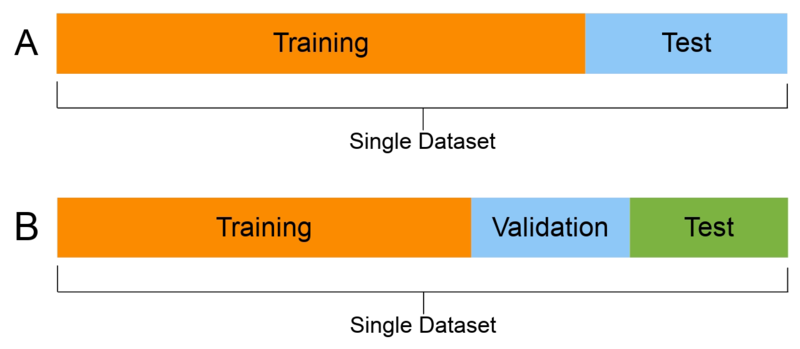
\includegraphics[width=0.8\linewidth]{fig/dataset.png}
    \caption{การแบ่งชุดข้อมูลทั้งหมดออกเป็น (A) Training Set และ Test Set และ (B) Training Set, Validation Set และ 
    Test Set (เครดิตภาพ: Wikimedia Commons)}
    \label{fig:dataset}
\end{figure}

ภาพที่ \ref{fig:dataset} แสดงสัดส่วนแบบคร่าว ๆ ในการแบ่งชุดข้อมูลออกเป็น Training Set และ Test Set และแสดงการแบ่งชุดข้อมูล%
อีกครั้งให้เป็น Training Set ที่จะถูกนำไปใช้ในการฝึกสอนโมเดลจริง ๆ และ Validation Set ที่จะถูกนำมาทดสอบโมเดลเพื่อเป็นการหยั่งเชิง%
ความสามารถของโมเดลก่อนที่จะนำไปใช้ทำนายค่าของ Test Set\footnote{โดยทั่วไปแล้วหลาย ๆ คนมักจะทำการแบ่งโดยใช้อัตราส่วนคือ 
80\% และ 20\% ตามหลักการของ Pareto \url{https://en.wikipedia.org/wiki/Pareto_principle}}

แล้วขั้นตอนการลด Bias นั่นมันเกิดขึ้นได้อย่างไร คำตอบก็คือในการแบ่งข้อมูลออกมาเป็น Validation Set (เช่นแบ่งออกมา 20\% จากทั้งหมด)
โดยทำการสุ่มเลือกบางส่วนของข้อมูลออกมา ซึ่งถ้าหากเราทำวนไปแบบนี้ไปเรื่อย ๆ เราจะเรียกว่าเป็นการทำ Validation แบบข้ามไปมาทั่วทั้ง 
Training Set ซึ่งเมื่อเรานำ Training Set แต่ละชุดไปฝึกสอนโมเดล เราจะได้ประสิทธิภาพของโมเดลแบบเฉลี่ย เปรียบเสมือนเป็นการเกลี่ย% 
หาความเท่ากันของข้อมูลนั่นเอง (กระจายออกไปให้เสมอกัน) ท้ายที่สุดแล้วถ้าเราแบ่งชุดข้อมูลตามที่ได้อธิบายมา เราจะมีอัตราส่วนของชุดข้อมูล%
ย่อย ๆ แต่ละประเภท ดังนี้

\begin{itemize}
    \item Training: 60\%
    \item Cross Validation: 20\%
    \item Testing: 20\%
\end{itemize}

%--------------------------
\subsection{ขั้นตอนการสร้างชุดข้อมูล}
\label{ssec:step_create_database}
\idxth{ชุดข้อมูล!ขั้นตอนการสร้างชุดข้อมูล}
%--------------------------


%--------------------------
\subsection{การสร้างชุดข้อมูลเคมีควอนตัม}
\label{ssec:step_create_qm_database}
\idxth{ชุดข้อมูล!การสร้างชุดข้อมูลเคมีควอนตัม}
%--------------------------
